\chapter*{LINUX Y LA EDUCACIÓN}
GNU/Linux es un sistema operativo de uso libre con una gran
variedad de funcionalidades que permite a los usuarios estar en
constante interacción con las aplicaciones que brinda, de
manera que puedan tanto visualizar como modificar los códigos
fuentes implementados por cada programador. Esto supone en
contrariedad con el software privado, una mayor fuente de
conocimiento que no inhibe ni limita el anhelo por leer codigo.

No se trata de sustituir un sistema operativo por otro porque ,
tal vez, sea más barato, seguro y fiable, sino de transmitir el
espíritu de colaboración y cooperatividad que es base de toda
empresa de conocimiento. El software libre es inherente a la
educacion por los valores que le guardan.

El software libre permite a los usuarios la libertad de controlar
sus ordenadores, y cooperar unos con otros sin tener
restricciones de ninguna índole. Además que supone un ahorro
significativo a la hora de copiar y redistribuir el software dentro
del sistema educativo.

Pero lo mencionado anteriormente es secundario al verdadero
objetivo por el que linux deber ser considerado un medio virtual
de aprendizaje significativo en constante evolución, esto es, la
implementación del uso continuo de software libre, no como un
sistema operativo que mejora la educación, sino que reemplaza
una educación limitada por una global y extendida.

Ahora analicemos cuestiones más profundas que nos permitiran
comprender el error en el que esta sometida nuestra sociedad
educativa, y por tanto, inculcada a los estudiantes.
La mision social de las escuelas es enseñar a ser ciudadanos de
una sociedad fuerte, independiente, capaz y libre; ¿libre?, esta
es la palabra clave en la cual debemos cuestionarnos y
preguntarnos , ¿qué clase de libertad tengo, si me cohiben de
ser empírico a la hora de extender mi conocimiento, visualizando
comportamientos internos de programas de gran importancia en
el mundo virtual?. Por ende el sistema educativo debe promover
el uso de software libre como promueven el voto.

Enseñando el software libre, pueden formar ciudadanos
integrales preparados para vivir en una sociedad digital libre de
yugos, a los cuales, las megacorporaciones nos quieren someter.
Por el contrario, al enseñar el uso del software no libre (privado
y de pago), se inculca la dependencia, lo cual se opone a la
misión de las empresas de conocimiento.

El software libre anima a todos a aprender: este repudia la
“encriptación de la tecnología y el saber” que mantiene a los
usuarios en la ignorancia del funcionamiento de la tecnología.
Por el contrario, el software privado abstiene a los usuarios de
adquirir conocimiento empírico.

El software libre en la educación es un medio interactivo para
enseñar y difundir el conocimiento en las escuelas; emitiendo
valores importantes como la solidaridad, libertad y trabajo
colaborativo; Solidario debido a que el usuario puede hacer
copias y distribuirlos libremente, al igual que modificarlas y
difundir diferentes versiones, cooperando al desarrollo
educacional de la comunidad.

La libertad del usuario es la mayor característica en el software
libre; puedes ejecutar el programa como desees, estudiar el
código fuente, cambiarlo y acomodarlo a tus necesidades y
gustos. Respecto al trabajo colaborativo se ve reflejado en las
miles de aplicaciones y obras libres, disponibles para usar,
copiar y modificar; esto hecho por personas de todo el planeta
con el ánimo de colaborar en la educación, el trabajo
comunitario y colaborativo.

El software libre significa un ahorro económico para los
institutos de enseñanza, además contribuirán al progreso de los
más brillantes en programación; los jóvenes despiertan a una
temprana edad un gran interés por saber todo acerca de la
computación y para ello es necesario leer código, modificar y
aportar nuevas ideas; y el software libre ofrece esta
oportunidad.
Pero sin duda la razón más profunda para utilizar software libre
en las escuelas es la educación moral, es enseñar a ser
ciudadanos; en el entorno informático esto se traduce en
instruir a compartir el software. 
Citando las palabras de Richard Stallman, “si traéis software a la escuela, debéis
compartirlo con los demás compañeros, y debéis mostrar el
código fuente en clase, por si alguien quiere aprender. Por lo
tanto, no está permitido traer a la escuela software que no sea
libre a menos que sirva para hacer un trabajo de ingeniería
inversa”.

Ocultar el conocimiento nunca ha formado parte de los
manuales ni la ética profesional, es la búsqueda dinámica y
transparente del conocimiento lo que se comparte por la
comunidad, pues es su mayor activo económico y cultural.
Existen grupos de usuarios muy activos y organizados que se
ayudan entre sí. Si uno tiene un problema puede dirigirse a ellos
para tratar de resolverlo.
Es un sistema seguro y fiable, el alumno no puede dañar el
sistema ni voluntaria, ni accidentalmente. Los niveles de
seguridad son muy altos tales que no será necesario reinstalar el
software.

\section*{ALGUNOS PROGRAMAS EDUCATIVOS IMPLEMENTADOS EN GNU/LINUX}
\subsection*{DEBIAN-JUNIOR}
Personalización de Debian para niños.
Consiste en ayudar a los niños en su proceso de familiarización
con el sistema operativo de manera que puedan adquirir algunas
habilidades y experiencias que tenemos como adultos, ademas
de transmitirles algunos valores como el amor por la libertad y
el fuerte sentido de comunidad.
Algunos beneficios y características de esta distribucion de linux
son:
1. Elegir un tema de escritorio y fondo.
2. Creación personalizada para niños pequeños de entornos de
escritorio.
\subsection*{EDUBUNTU}
Distribucion basada en Ubuntu.
Es una derivación oficial de la distribucion Linux Ubuntu
destinada para ambientes escolares, desarrollada por docentes y
tecnólogos de diferentes países, esto, con el objeto de tener
varias perspectivas de las metodologías pedagógicas que se
utilizan para el aprendizaje de población de entre 6 y 18 años.
La ultima version de esta distribucion es Edubuntu 13.04.

Los objetivos principales de Edubuntu son crear una
centralización administrativa de todos los procesos, usuarios y
demás configuraciones, de un laboratorio de cómputo, con el fin
de poder trabajar en un ambiente de colaboración en clase.
Ademas de coleccionar el mejor software libre con fines
educativos.

\subsection*{EDULINUX}
Distribucion basada en Ubuntu creada por el
Ministerio de Educación de Chile y el Instituto de Informática
Educativa.
Esta distribucion surgió por la necesidad de reutilizar
computadoras antiguas instaladas en la Red Escolar Enlaces de
Chile.

Se materializo a traves una Distribucion Educativa del Sistema
Operativo Linux, que contiene un grupo de aplicaciones libres,
para internet, software de ofimática, un paquete de software
educativo que proviene del proyecto KDE Edutaiment, entre
otros paquetes. Esta distribucion consiste en un sistema
cliente /servidor que funciona a traves de un computador
potente (servidor); potente en el sentido de que posee un
procesador multinucleos, memoria aleatoria y disco duro de
gran capacidad, etc. Y diversos computadores antiguos(clientes),
que conectados todos al servidor, se genera un mayor
aprovechamiento, que por si solos no pueden utilizar aplicacion
modernas.

\subsubsection*{ALGUNAS CONTROVERSIAS POR SU NOMBRE}

Se suele confundir esta distribucion con otra, de origen
canadiense, antiguamente denominada EduLinux, pero que
actualmente se denomina LinuxEdu-Québec.
Por otro lado, existe otra distribucion de origen polaco
denominada LinuxEdu-CD.

\subsection*{LIHUEN}
Distribucion basada en Debian creada por la
Universidad Nacional de la Plata en Argentina.
Esta orientada a escritorios educativos y destinada para
computadores con arquitecturas de 32 a 64 bits del proyecto
Conectar igualdad y similares.
La última versión de Lihuen es la 4.0.1.
A partir de la versión 3.0, Lihuen comenzó a utilizar una
modificacion del instalador Debian; ya que en versiones
anteriores utilizaba Anaconda.
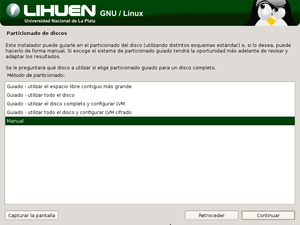
\includegraphics[scale=0.5]{img/cp06/img0601.png}
\subsection*{LULA}
Distribucion basada en Ubuntu destinada para
universidades latinoamericanas.
Este proyecto inicio en el año 2009 con la participacion de
tecnologicos y educadores de las universidades que componen el
CAVILA (campus virtual latinoameticano).

Fue una iniciativa sin ánimo de lucro desarrollada en la Red de
Catedras Telefonica con el objetivo de integrar el software libre
en las universidad latinoamericanas y por ende en la docencia.
Se caracteriza por recopilar el mayor numero de aplicaciones
educativas usadas en el ámbito pedagógico; ademas que los
profesores tienen la posibilidad de conocer las aplicaciones que 
utilizan sus colegas de docencia, y asi mismo implementar
metodologías de estudio netamente virtuales.

\subsection*{MAX}

Distribucion creada por la consejeria de Educacion de la
Comunidad de Madrid, España. Desde sus inicios se ha basado
en Ubuntu GNU/Linux. Su último lanzamiento fue el 18 de
noviembre del 2012 con la version MAX 7.0 basada en Ubuntu
12.04 LTS.
MAX es una distribucion educativa que alverga un gran conjunto
de de programas instructivos, ademas de programas de
escritorio habituales.
las principales características de MAX son su sencillez,
estabilidad y gran colección de aplicaciones.
MAX puede ser instalado mediante un DVD o USB.

\subsection*{SKOLELINUX/DEBIAN-EDU}
Es una completa y libre solución de
software para las escuelas, ya que reduce los costos, prolonga la
vida de utilidad del hardware y cubre una gran multiplicidad de
aspectos de las escuelas en el ámbito pedagógico.
El objetivo de esta personalización de Debian es hacer que sea
facil y atractivo a la hora de ser instalado; ademas de
proporcionar una gerencia administrativa con respecto a todas
las aplicaciones utilizadas por el estudiantado.
SkoleLinux contiene varios servicios a la hora de ser instalado,
entre otros:
\begin{itemize}
  \item Catálogo central de usuarios: Un usuario y clave para
        administrar varias maquinas.
  \item Almacenamiento central: Siempre habrá una interfaz facil de usar, sin importar que maquina dentro de la conexión de red esté usando.
  \item Posibilidad de compartir las impresoras en distintos puntos de la red.
\end{itemize}

La ultima version que ha salido de esta distribucion fue lanzada
el 28 de septiembre del 2013 llamada SkoleLinux 7.1(o tambien
denominada Debian Edu 7.1 + edu0 ) basado en debian wheezy.

\subsection*{EHUX}
Es un proyecto basado en GNU linux Kubuntu de la
universidad del país vasco.
El objetivo de EHUX es que absolutamente todo el alumnado de
la universidad conozco LINUX y sus ventajas dentro del campus,
de manera que por medio de esta distribucion se desarrollen
todas las funciones informáticas requeridas en cualquier
carrera.

\subsection*{LINKAT}
Es una distribucion basada en GNU/LINUX creada por el
departamento de educación de la generalidad de cataluña. Se
apoya en la distribucion OPENSUSE(proyecto libre auspiciado
por SUSE Linux GmbH y AMD) y la ejecución de los programas
se basa en paquetes rpm(herramienta de administracion de
paquetes pensada en GNU/LINUX).
La ultima version de esta distribucion por el momento es la 4.0
basada en el entorno de escritorio Gnome, pero tambien
disponible en entornos KDE y XFCE.
Sus principales características son:

\begin{itemize}
  \item Contiene una gran cantidad de herramientas y aplicaciones de comunicacion y creacion.
  \item Admite que cualquier persona en calidad de usuario forme parte activa en el desarrollo y mejora de la distribucion.
  \item Se actualiza automaticamente.
  \item Procede de OPENSUSE.
\end{itemize}

\subsection*{GUADALINEX}
Es un sistema operativo basado en GNULinEX
creado por la Junta de Andalucía destinado para dar
cumplimiento al decreto 72/2003, en donde se opta por el el uso
de software libre como medio para impulsar el potencial de
conocimiento en Andalucía.
Caracteristicas:

\begin{itemize}
  \item Su contenido esta en español.
  \item Incluye todas las aplicaciones y herramientas para ser un sistema operativo libre y completo(suite ofimática, reproductores multimedia, editor de diseño gráfico, aplicaciones para desarrollo , etc).
  \item Posee la interfaz gráfica por defecto Gnome Shell.
  \item Inclusión de la aplicacion control parental Nanny, que consiste en la gestión del internet, limitando el tiempo de para cada usuario del PC y controlando el bloqueo de paginas web no deseadas.
  \item Dispone de soporte tecnico gratuito para los usuarios de Guadalinex.
\end{itemize}

\section*{ALGUNAS CRÍTICAS AL SISTEMA}

El obstáculo más frecuente es el factor de compatibilidad entre
el sistema operativo y el hardware. Hay pocos proveedores de
sistemas físico computacionales (hardware) que prolongan
controladores (o también llamados drivers) para sus
ofrecimientos en el mercado de demanda (en la mayoría de los
casos, estos controladores son mantenidos y adaptados a los
diversos sistemas operativos por fanáticos). No obstante, la
única salida real es obtener el listado de hardware que soporta
cada distribucion, y por tanto, los componentes adaptativos a
cada sistema físico.

Actualmente, hay empresas de talla mundial como Compaq e
IBM, que exportan equipos con linux preinstalado, lo que
favorece la ductilidad del sistema operativo con el hardware y
sus componentes.

En general, la variedad de hardware que soporta Linux es
mucho más extensa que la que soportan versiones comerciales
de Unix, debido a que cualquier fanático está en las condiciones
de crear el soporte requerido para cualquier dispositivo ajeno a
este sistema operativo y aportarlo a la versión oficial(ademas de
la popularidad con la que cuenta este S.O).

Otra crítica, es que hay pocas empresas que se dedican al
desarrollo de aplicaciones para linux. En contraparte, hay una
gran oferta en el mercado de software para una significativa
variedad de lenguajes tradicionales, pero en el área de
desarrollo de ambiente gráfico oferta es muy pobre.

También se ha criticado la carencia de ambientes graficos para
linux, pero actualmente este limitante se ha solucionado a través
de KDE y Gnome (ambos entornos de escritorio).

\section*{RECURSOS Y APLICACIONES EDUCATIVAS PARA LINUX}
En linux se puede encontrar una gran variedad de herramientas
como :
\begin{itemize}
  \item Navegadores
  \item Transferencia de archivos
  \item Editores de texto
  \item Herramientas de oficina
  \item Hojas de cálculo, etc.
\end{itemize}
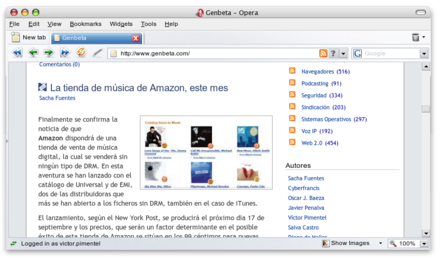
\includegraphics[scale=0.5]{img/cp06/img0602.png}

Ademas, que es bastante sencillo y cómodo instalar nuevas
aplicaciones, ya que no hay una sola forma de hacerlo, sino que
hay múltiples alternativas como agregar o quitar programas,
desde la terminal de linux, o bajandola desde algún directorio.
En esta última es donde se hará énfasis, ya que es de profunda
necesidad conocer de lleno las opiniones, comentarios, notas
tecnicas y clasificación de cada aplicacion. Estos son algunos
directorios de aplicaciones para sistemas de código abierto:
\begin{description}
	\item[ OFFSETs Freeduc:] Brinda un directorio que permitirá encontrar
	de manera rápida cualquier aplicacion útil para las escuelas.
	\item[ Ohloh:] Es una red social de aplicaciones, que tiene como
	objetivo fundamental poder conectar de manera múltiple
	usuarios con el software que usan y/o proyectos libres que
	crean.
	\item[ Getdeb:] En este directorio se encuentra todo tipo de programas
	para descargar en archivos DEB.
	\item[ Open Source Living:]Es tal vez un directorio popular, conocido
	por una gran variedad de personas, que permite localizar
	aplicaciones cómodamente, debido a que las ordena de manera
	jerarquica.
	\item[ KDE Edutainment:] Diseñado para la creación de software de
	código abierto basado en KDE (comunidad internacional que
	desarrolla software libre).Además que entrega aplicaciones para
	ser utilizadas por docentes.
\end{description}

\section*{VENTAJAS DEL USO DE SOFTWARE LIBRE EN LA EDUCACIÓN}
\begin{itemize}
  \item El código es abierto: Permite reutilizar código a partir de
	las aplicaciones creadas para adaptarlo a nuevas
	necesidades o tomarlo como referencia para la creacion
	de nuevas aplicaciones. Por ejemplo, adaptar una
	aplicacion a un ambiente gráfico ameno a las necesidades
	de un determinado grupo de estudiantes.
  \item Colaborativo: El prototipo de desarrollo es participativo.
  \item La copia es legal: Tanto docentes como alumnos pueden
	redistribuir copias del mismo legalmente. Asi se evita la
	pirateria.
  \item Resistencia a los virus: Existen cerca de 6 virus conocidos
	para GNU/Linux, mientras que en otros sistemas
	operativos la estadística de virus cada vez es más
	creciente. Puede pensarse que linux no es un sistema
	operativo muy utilizado para ser blanco de “crackers”,
	pero esto es solo un factor minucioso, ya que el diseño de
	este, permite que el hacer virus sea una tarea bastante
	complicada.
  \item Permite reutilizar equipos: Admite que equipos que han
	sido dejados a un lado ya sea por el surgimiento de
	nuevas tecnologías o incapacidad de realizar ciertas
	tareas puedan volver a ser utilizados por medio de
	tecnologías que permitirán volverlos operativos con un
	alto nivel de productividad.
  \item Multiplataforma: Plataformas soportadas por la
	distribucion GNU/Linux:
	1. Procesadores Alpha de DEC.
	2. Procesadores IA-32 elaborados por Intel, AMD, Cyrix y otros.
	3. Computadoras personales, Apple Macintosh, Atari y Amiga.
	4. Maquina NetWinder.
	5. Estaciones de trabajo Sun UltraSPARC.
	6. Arquitectura PA-RISC de Hewlett-Packard.
	7. Arquitectura de 64 bits de Intel.
\end{itemize}

\section*{LINUX EN LA EDUCACIÓN SUPERIOR}
Hoy en dia es notable el uso frecuente de tecnologias de
informacion y las comunidades al proceso curricular. La
universidad no puede ser tercera a los desafíos que impone la
sociedad de la informacion para permanecer activa a los avances
tecnológicos, y vincularlos a una academia en excelencia.

El software se ha convertido en una metodología pedagógica
que virtualiza y digitaliza toda la información requerida para el
aprendizaje.

El software, a lo largo del tiempo se ha venido convirtiendo en
una mercancía que representa el egoísmo y la ambición de las
empresas, ya que la naturaleza neta del software anteriormente
era de libertad. Al punto que hoy en día, se desata una perpetua
lucha de subsistencia en las economías mundiales.

El software, un elemento reproducible sin límite, ha sido
convertido en un producto escaso y negociable, que estaría
refutando el principio que alude : “El conocimiento es el único
bien que más crece cuanto más se comparte ”. De esta manera
el conocimiento englobado del software se privatizó en derechos
de autor reservados o también llamada copyright.

\includegraphics[scale=0.5]{img/cp06/img0603.png}
En la actualidad, la universidad, cuna del conocimiento se
encuentra en un dilema de usar y enseñar con un software que
no puede estudiar a fondo ni compartir, o encontrar un camino
para el que el software no sea visto como una mercancía sino
como conocimiento.

A este problema se enfrentó Richard Stallman, un investigador
del Instituto Tecnologico de Massachusetts(MIT),cuando le
pidieron firmar un acuerdo de no divulgación que violaba sus
principios y preceptos morales. En 1983, inició un proyecto
denominado GNU que buscaba la creacion de un sistema
operativo libre y que fuera alternativa al sistema operativo
UNIX. Posteriormente, esto lo llevó a escribir el “Manifiesto
GNU”, que sería la raíz y base de una filosofía que daría
surgimiento al Movimiento del Software Libre.

Stallman planteo 4 principios sobre los cuales se fundamenta la
libertad y verdadera esencia de los usuarios sobre los
programas. Estos se resumen:

El programa pueda ser estudiado y modificado. Que se pueda
distribuir y copiar sin tapujo alguno. Que pueda ser mejorado.
Que pueda ser ejecutado de acuerdo a los propósitos del
usuario.

Estos preceptos coinciden con la moral y la ética de las
empresas del conocimiento.

Ademas hay razones, por las cuales la educación no debería usar
software que va en contra las libertades del software libre.

Razón moral: La educación básicamente enseña a los
estudiantes que empresa productora de software es más
eficiente para utilizar como recurso (convirtiéndonos más en
clientes que en innovadores), más que , el de enseñar conceptos
y fundamentos de las herramientas que utilizan.

Razón social: Es un prototipo basado en la cooperatividad social,
que contrasta con los modelos de sustentabilidad de la sociedad.

Razon economica: La libertad de poder distribuir y copiar sin
impedimento alguno, implica un ahorro significativo a la hora de
legalizar software en cualquier institución del conocimiento;
luego, no será necesario dar excedentes o algún pago, para
obtener actualización contiguas de los programas que se
utilicen. En contraposición con el software privativo, este más
bien se considera como un producto más que como una
herramienta de conocimiento, ya que al pagar de manera
significativa esas licencias, adquirimos no la propiedad sino el
derecho de poder usar ese programa. con ese dinero se podría
destinar a necesidades más imperiosas como lo es la educación.

Razón temporal: El software libre permite manipular y observar
su código y funcionamiento incorporado, lo que implica que , el
software es independiente a la empresa que lo creo, ya que si
llegase por algún momento a extinguirse la empresa, el software
podrá ser mantenido y actualizado por la comunidad de software
libre.

Razon legal: No hay alguna ley constitucional que impida o
limite la manipulación y/o redistribución del software libre.

\section*{OLPC (UN COMPUTADOR POR CADA NIÑO)}

El proyecto OLPC nace en el año 2005, en el Media Lab de MIT
(Laboratorio de Medios del Instituto Tecnológico de
Massachussets, EEUU), es un proyecto centrado en la entrega
de un portátil de bajo costo, fabricado con el propósito de
proporcionar a cualquier niño del mundo conocimiento y acceso
a la tecnología de la información como forma moderna de
educación; Una de sus características más importantes es que
las computadoras deben ejecutar únicamente software libre. Es
así que nace la organización sin fines de lucro denominada “One
Laptop per Child (OLPC – Un computador por cada niño)” que es
independiente del MIT.

El proyecto cuenta con el apoyo y la colaboración de Google,
AMD, Red Hat, News Corp, Brightstar Corp y otras empresas.
Para elaborar computadores portátiles de bajo costo, bajo
consumo de energía, con los requisitos necesarios para trabajar
en condiciones extremas y áreas remotas, debido a que el
proyecto esta principalmente enfocado a las zonas rurales en
vías de desarrollo donde los niños cuentan con muy poco
material para estudiar, aprender y avanzar en un mundo
tecnológico. La idea básica es acercar a cada niño a un
computador para que lo pueda utilizar ya sea en el aula como en
su hogar. Se trata de que cada niño se “apropie” de “su”
computador y lo utilice ya sea en el aula como en su casa, de
igual manera que lo haría con un libro de textos.
Posee programas preinstalados para que cada niño pueda crear,
aprender, explorar escribir, dibujar, entrar a internet, jugar,
escuchar música, tomar fotos etc.
Existen 5 condiciones de usos para todo aquel que obtenga un
computador portátil:

1. Los niños conservan los computadores portátiles.
   Son libres de llevar sus computadores a casa, al colegio o
   a cualquier lugar donde ellos deseen.

2. Enfoque en la educación temprana.
   Niños de 6 a 12 años de edad.

3. Sin dejar a ninguno fuera.
   Se suministran un gran número de computadores
   portátiles en colegios y fundaciones sin dejar a ninguno
   fuera.
   
4. Conexión a internet.
   Los usuarios pueden acceder a internet desde casi
   cualquier sitio en donde se encuentren.
   
5. Crece y se adapta a las necesidades del niño.

El proyecto OLPC intenta introducir un cambio radical en la
manera de plantear las actividades a los alumnos, tanto las que
se deban realizar en clase como en el hogar. Se trata de que los
niños se “apropien” de las computadoras y puedan acercar la
tecnología también a sus hogares.

Este proyecto es sumamente actual y requiere una gran
responsabilidad a la hora de la elección del software de base y
de las aplicaciones contenidas en él, como también de las
actividades pensadas para su uso.

Este artículo presenta las distintas líneas de investigación
llevadas a cabo en el LINTI, en donde se espera continuar con
este análisis y concluir con una propuesta definitiva tanto de
software como de usos educativos de la OLPC.

Esto dijo Kofi Annan (secretario general de la ONU), "Esto no es
sólo una cuestión de dar un ordenador portátil a cada niño,
como si otorgar el cual amuleto mágico. La magia está dentro -.
Dentro de cada niño, en cada científico, estudioso, o
simplemente ciudadano normal en la toma de esta iniciativa.
Tiene la intención de que eso salga a la luz del día. "
   
\section*{DISTRIBUCIONES GNU/LINUX HECHOS EN MÉXICO}
Al programa de usuario, programa y núcleo (kernel) del sistema,
a todo este conjunto se le conoce como distribución.
\subsection*{GOBIERNO GNU/LINUX}
Es inicialmente un proyecto planteado por la subdirección de
informática delegación de Tlaplan para pasarse al software libre.
Como primer objetivo en el que pensaron, fue en crear un 
sistema operativo basado en Fedora (una colección de software
fundamentado en Linux que hace funcionar a su computador).
Este tiene que cumplir con los requerimientos que requiere el
gobierno del Distrito Federal, que contribuya al fortalecimiento
del programa de migración hacia el software libre y que sea una
herramienta de expansión a la comunidad en general.
Según la página de internet del proyecto las ventajas de instalar
esta distribución en el gobierno son:
\begin{itemize}
  \item Ahorro de entre $6,000 y $9,000 por computadora, por
	gastos en compra de licencias y activaciones.
  \item Beneficio social.
  \item Beneficio tecnológico.
  \item Combate efectivo en la copia ilícita del software.
  \item Eliminación de barreras presupuestales.
  \item Reutilización de sistemas desarrollados.
\end{itemize}
La distribución trabaja bajo un kernel versión 2.6.11. Las
herramientas que contiene esta distribución entre otras
son:
\begin{itemize}
  \item Firefox 1.0.4
  \item Openoffice 2.0
  \item Samba 3.0.14
  \item Gcc 4.0
  \item Gnome-desktop 2.10.0
  \item Php-5.0.4
  \item Perl-5.8.6
  \item Python- 2.4.1
  \item Postgresql-8.0.3
\end{itemize}
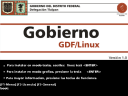
\includegraphics[scale=0.5]{img/cp06/img0604.png}
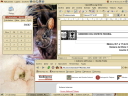
\includegraphics[scale=0.5]{img/cp06/img0605.png}

Acontinuacion se exponen algunas de las distribuciones hechas
por universidades, instituciones o grupos que trabajan con
GNU/Linux.

\subsection*{BEAK OS}
La idea de la distribucion BeakOS, inicia tras analizar la
tendencia de otras distribuciones de GNU/Linux al intentar
acercarse más al usuario final, incluyendo a éstas en sus
aplicaciones, interfaces gráficas. BeakOS es un sistema
desarrollado en software libre impulsado por infotec y
totalmente gratuito para desempeñarse en ambientes de
producción.

Caracteristicas:
\begin{itemize}
  \item No esta basado en ninguna distribucion de GNU/Linux
  \item Bajo consumo de recursos
  \item Libre distribucion bajo los términos de GPL
  \item Rapidez y confiabilidad
  \item Facil administracion a traves de interfaces web
\end{itemize}

\subsection*{ALDOS 1.4}
Es un sistema operativo con soporte de largo plazo y
estrictamente orientado para el uso, como el sistema operativo
de escritorio. Joel Barrios Dueñas es el desarrollador, diseñador
y encargado del mantenimiento de este sistema operativo, a
través de alcance libre. que decidieron hacer una versión del
sistema GNU/Linux sin tantos programas, más ligera pero sin
renunciar a las mejores aplicaciones y entornos de escritorio.
En la página oficial de alcance libre se mencionan las
características:

\begin{itemize}
  \item Linux Standard Base 4.0
  \item Núcleo 3.4 LTS (maquillado como 2.6.44.x para fines de
	compatibilidad)
  \item GNOME 2.32 con muchas mejoras implementadas por
	AlcanceLibre.org
  \item X11R7.7 con X server 1.12
  \item Firefox edición ESR (Extended Support Release)
  \item Thunderbird edición ESR (Extended Support Release)
  \item LibreOffice (se instala versión 3.6 y actualiza a la 4.1)
  \item SELinux desactivado de modo predeterminado para
	economizar recursos
  \item IPv6 activo de modo predeterminado
  \item De modo predeterminado, sólo se instala localización para
	español, catalán e inglés para economizar espacio en
	medios de almacenamiento
  \item Mínimo de servicios de arranque para lograr un inicio
	rápido
  \item GNOME Mplayer como reproductor de medios
	predeterminado
  \item Soporte multimedios completo para formatos privativos
	de audio y video en GNOME Mplayer
  \item Soporte para MP3 y otros formatos privativos de audio en
	Rhythmbox
  \item Pidgin como cliente de mensajería instantánea
	predeterminado
  \item En los almacenes YUM de ALDOS hay más de 8870
	paquetes, entre los que se incluyen Gimp 2.8, VirtualBox
	4.2, Inkscape 0.48.x, controladores de Nvidia 96xx, 173xx
	y 304, Catalyst 12.4 y 12.10, docenas de juegos y mucho
	más
\end{itemize}

\subsection*{JARRO NEGRO}
Para hablar del jarro negro primero tenemos que mirar un poco
el proyecto muser, que intentaba desarrollar una distribucion
para servidores de diferentes arquitecturas (en particular
SPARC). cuando llevaban un avance del proyecto (un LiveCD de
10MB) decidieron elaborar una distribucion para el plantel.
Jarro Negro es el nombre de esta distribucion GNU/Linux
desarrollada en Mexico por alumnos y profesores del Colegio de
Ciencias y Humanidades (CCH), de la Universidad Nacional
Autónoma de México (UNAM).

Contiene reproductores de audio y video, OpenOffice,
compiladores, navegadores y mensajeros instantáneos.

Caracteristicas:

\begin{itemize}
  \item Gestor de ventanas Enlightenment
  \item Kernel 2.6.27
  \item Openoffice2
  \item Firefox 3 (Con Flash, Java y Mplayer plugins)
  \item Java JRE 1.6
  \item Gtk 2.12.11
  \item Mplayer (Con w32codecs)
  \item PcMan File Manager 0.5
  \item Entre otras . . .
\end{itemize}

\section*{LEYES SOBRE SOFTWARE LIBRE EN COLOMBIA}

Ley 11723: Es la ley conocida como “Ley de propiedad
intelectual” compuesta por 89 artículos (actualmente vigente).
Esta ley regula todo lo que compete a derechos de propiedad
sobre alguna obra artística, científica o literaria,
enajenación,etc. que de incurrir en contra de esta norma, puede
haber sanciones tanto pecuniarias(multa) como carcelarias.

Su última reforma fue en Noviembre de 1998, cuando por ley
25036 se le introdujeron actualizaciones debido a la
especulación de que si el software como producto se encontraba
bajo amparo de esta ley. Ahora establece en el artículo 1: “Los
autores de obras literarias, científicas y artísticas gozarán de
protección para sus obras en la forma prescrita por la presente
ley y, en cuanto fuere compatible con ella, por el derecho común.
También protege esta ley a los intérpretes o ejecutantes, a los
productores de fonogramas y a los organismos de radiodifusión,
en sus derechos conexos a los del autor” y en su artículos 55: “
La explotación de la propiedad intelectual sobre los programas
de computación incluirá entre otras formas los contratos de
licencias para su uso o reproducción ”.

Proyecto de ley sobre el software libre: Es un proyecto
presentado por el parlamento (más exactamente por Marcelo
Luis Dragan) a principios del año 2002 para adoptar la
posibilidad por parte de colombia de adquirir una legislación
que regule de manera general las políticas de uso y empleo del
software libre tanto en entidades gubernamentales como en
empresas donde existan una cantidad significativa de acciones
por parte del estado.

Entre las causas que motivaron al proyecto hay mayor énfasis en
el moral (no es desconocimiento para nadie que en todos los
ámbitos de la administración pública se utiliza software sin
licencia legal ya sea por falta de recursos o rebeldía), el
económico(por el costo de las licencias), el educativo, cultural,
etc.

El proyecto consta de 21(veintiuno) artículos que regulan
conjuntamente los sistemas de información evitando ser
dependiente de la empresa que lo creó, promoviendo la igualdad
en el acceso a la información pública, evitar el acceso a la
información por parte de terceros no autorizados según la
constitución.

De acuerdo al literal c del artículo 1 del proyecto se entra a
aclarar lo que se puede y no se puede definir como software
libre en tanto cumpla las siguientes libertades:

\begin{itemize}
  \item Libertad de ejecutar para cualquier propósito el
	software(sin imponer restricciones)
  \item Libertad de estudiar el funcionamiento interno del
	programa
  \item Libertad para redistribuir copias del programa
  \item Libertad de modificar el programa y publicar sus
	actualizaciones al público bajo las mismas condiciones del
	programa original
\end{itemize}

Es importante resaltar que el software libre no atenta contra los
derechos de autor ni de propiedad intelectual, no exaltando así
la piratería, ya que en tanto los autores autorizan a los demás
hacer uso de su software ofreciendo las libertades de la filosofía
de software de código abierto.

Otro aspecto relevante, es el de permitir a los usuarios estudiar
y modificar el código fuente del programa, generando así un
avance significativo en el software libre. Cualquier persona con
conocimientos técnicoss de programación, puede fácilmente
adaptar a sus necesidades y aumentar las capacidades del
software.

\subsection*{RAZONES CONSTITUCIONALES}
Este proyecto aparte de incentivar el desarrollo tecnologico de
los sistemas de información y contribuir a la seguridad nacional,
se basa en los principios y valores por los que debe luchar el
estado.

Segun el artículo 15 de la constitución política de colombia :
“Todas las personas tienen derecho a su intimidad personal y
familiar y a su buen nombre, y el Estado debe respetarlos y
hacerlos respetar. De igual modo, tienen derecho a conocer,
actualizar y rectificar las informaciones que se hayan recogido
sobre ellas en bancos de datos y en archivos de entidades
públicas y privadas.” Ademas el articulo 74 de la misma : “Todas
las personas tienen derecho a acceder a los documentos
públicos salvo los casos que establezca la ley.”. Por ende los
datos en donde haya confidencialidad debe tener un trato
especial ya que ha ellos solo podrá haber acceso directo para
instituciones estatales u organismos autorizados.

El software que sea utilizado por el gobierno debería tener el
mismo trato que con las información pública, de manera que, se
pueda estudiar y analizar los procedimientos internos a la hora
de ser llevados a cabo.

\subsection*{EXPERIENCIAS DE SOFTWARE LIBRE EN COLOMBIA}
 
Desde principios de 1990 ,el impacto del software libre ya
estaba siendo asimilado por la sociedad, usándose tanto en
sector privativo como en el público. Ya se estaba instaurando
una filosofía de código abierto (Open source) que permitía el
desarrollo del movimiento de software libre.

El medio académico, científico y de investigación han sido el
medio más propicio para instaurar la filosofía del software libre
en colombia. La Universidad Nacional de Colombia, la Pontificia
Universidad Javeriana, la Universidad de los Andes, la
Universidad de Antioquia, la Universidad del Valle, la Escuela de
Administración de Negocios, la Universidad de Manizales, la
Universidad de san Buenaventura, la Universidad Distrital
Francisco José de caldas, la Universidad Industrial de Santander
y muchas más; siendo los ambientes más propicios donde el
movimiento del software libre han tenido mayor acogida.

En los sectores oficiales y privativos, también se ha mostrado un
avance significativo respecto al uso del software libre frente a
sus infraestructuras de datos, manejo de sus comunicaciones,
sitios web, conexión de sus equipos a la red y control del mismo.

En algunas instituciones estatales como la Armada Nacional, el
IDEAM, Telecom, la Defensoría del Pueblo, la Contraloría
General de la Nación y la Superintendencia de Industria y
Comercio usan software libre para objetivos semejantes a las
antes citadas.

En el 2003 el programa de ingeniería de sistemas de la
Universidad de los Andes, auspiciado por Sun Microsystems,
organizaron una jornada de software libre denominada
SOFTWARE LIBRE EN COLOMBIA: UNA REALIDAD; en ella,
asistieron personas de varias localidades del país, interesados
en el desarrollo tecnico del software libre en colombia. En esta
jornada, se presentó una visión general interesante y aplicada
de esta tecnología en colombia, exhibiendo una serie de
proyectos desarrollados por empresas que se dedican a la
informática, y a emprender cada día un nuevo aporte frente al
software GNU/linux.

En mayo del 2012, se realizó en Bogotá-colombia el festival
latinoamericano de instalación de software libre en el que
asistieron miles de colombianos con el fin de conocer las
experiencias de grupos, proyectos y comunidades que trabajan
con herramientas libres.

En este evento se vio reflejada la solidaridad de jóvenes con
conocimientos acerca del funcionamiento de Linux que por
propia voluntad se ofrecieron como conferencistas y/o
instaladores de las diferentes distribuciones de linux enseñando
el verdadero concepto de cultura libre.

Actualmente Linux es un núcleo monolítico híbrido. Los
controladores de dispositivos y las extensiones del núcleo
normalmente se ejecutan en un espacio privilegiado conocido
como anillo 0 (ring 0), con acceso irrestricto al hardware,
aunque algunos se ejecutan en espacio de usuario. A diferencia
de los núcleos monolíticos tradicionales, los controladores de
dispositivos y las extensiones al núcleo se pueden cargar y
descargar fácilmente como módulos, mientras el sistema
continúa funcionando sin interrupciones. También, a diferencia
de los núcleos monolíticos tradicionales, los controladores
pueden ser prevolcados (detenidos momentáneamente por
actividades más importantes) bajo ciertas condiciones. Esta
habilidad fue agregada para gestionar correctamente
interrupciones de hardware, y para mejorar el soporte
demultiprocesamiento simétrico.

El hecho de que Linux no fuera desarrollado siguiendo el diseño
de un micronúcleo (diseño que, en aquella época, era
considerado el más apropiado para un núcleo por muchos
teóricos informáticos) fue asunto de una famosa y acalorada
discusión entre Linus Torvalds y Andrew S. Tanenbaum.

En Linux existe un sistema de archivos que carga y contiene
todos los directorios, redes, programas, particiones, dispositivos,
etc. que el sistema sabe reconocer, o por lo menos, identificar.

Este sistema de ficheros y directorios, tiene como base al
carácter (/); ese mismo carácter sirve también para demarcar los
directorios, como por ejemplo: "/home/usuario/imagen.jpg". El
directorio especificado por una ruta consistente sólo por este
carácter contiene toda la jerarquía de los directorios que
constituyen todo el sistema. A este directorio suele llamárselo
directorio raíz. En Linux, a los discos no se les asigna una letra
como en Windows (p.e. "C:"), sino que se les asigna un directorio
de la jerarquía del directorio raíz (/), como por ejemplo:
"/media/floppy".




